%%%%%%%%%%%%%%%%%%%%%%%%%%%%%%%%%%%%%%%%%
% Short Sectioned Assignment LaTeX Template Version 1.0 (5/5/12)
% This template has been downloaded from: http://www.LaTeXTemplates.com
% Original author:  Frits Wenneker (http://www.howtotex.com)
% License: CC BY-NC-SA 3.0 (http://creativecommons.org/licenses/by-nc-sa/3.0/)
%%%%%%%%%%%%%%%%%%%%%%%%%%%%%%%%%%%%%%%%%

%----------------------------------------------------------------------------------------
%	PACKAGES AND OTHER DOCUMENT CONFIGURATIONS
%----------------------------------------------------------------------------------------

\documentclass[paper=a4, fontsize=11pt]{scrartcl} % A4 paper and 11pt font size

% ---- Entrada y salida de texto -----

\usepackage[T1]{fontenc} % Use 8-bit encoding that has 256 glyphs
\usepackage[utf8]{inputenc}
%\usepackage{fourier} % Use the Adobe Utopia font for the document - comment this line to return to the LaTeX default

\usepackage{eurosym}
\usepackage{multirow}
% ---- Idioma --------

\usepackage[spanish, es-tabla]{babel} % Selecciona el español para palabras introducidas automáticamente, p.ej. "septiembre" en la fecha y especifica que se use la palabra Tabla en vez de Cuadro

% ---- Otros paquetes ----

\usepackage{url} % ,href} %para incluir URLs e hipervínculos dentro del texto (aunque hay que instalar href)
\usepackage{amsmath,amsfonts,amsthm} % Math packages
%\usepackage{graphics,graphicx, floatrow} %para incluir imágenes y notas en las imágenes
\usepackage{graphics,graphicx, float} %para incluir imágenes y colocarlas

% Para hacer tablas comlejas
%\usepackage{multirow}
%\usepackage{threeparttable}

%\usepackage{sectsty} % Allows customizing section commands
%\allsectionsfont{\centering \normalfont\scshape} % Make all sections centered, the default font and small caps

\usepackage{fancyhdr} % Custom headers and footers
\pagestyle{fancyplain} % Makes all pages in the document conform to the custom headers and footers
\fancyhead{} % No page header - if you want one, create it in the same way as the footers below
\fancyfoot[L]{} % Empty left footer
\fancyfoot[C]{} % Empty center footer
\fancyfoot[R]{\thepage} % Page numbering for right footer
\renewcommand{\headrulewidth}{0pt} % Remove header underlines
\renewcommand{\footrulewidth}{0pt} % Remove footer underlines
\setlength{\headheight}{13.6pt} % Customize the height of the header

\numberwithin{equation}{section} % Number equations within sections (i.e. 1.1, 1.2, 2.1, 2.2 instead of 1, 2, 3, 4)
\numberwithin{figure}{section} % Number figures within sections (i.e. 1.1, 1.2, 2.1, 2.2 instead of 1, 2, 3, 4)
\numberwithin{table}{section} % Number tables within sections (i.e. 1.1, 1.2, 2.1, 2.2 instead of 1, 2, 3, 4)

\setlength\parindent{0pt} % Removes all indentation from paragraphs - comment this line for an assignment with lots of text

\newcommand{\horrule}[1]{\rule{\linewidth}{#1}} % Create horizontal rule command with 1 argument of height



%----------------------------------------------------------------------------------------
%	TÍTULO Y DATOS DEL ALUMNO
%----------------------------------------------------------------------------------------

\title{	
\normalfont \normalsize 
\textsc{\textbf{Ingeniería de Servidores (2016-2017)} \\ Grado en Ingeniería Informática \\ Universidad de Granada} \\ [25pt] % Your university, school and/or department name(s)
\horrule{0.5pt} \\[0.4cm] % Thin top horizontal rule
\huge Memoria Práctica 5 \\ % The assignment title
\horrule{2pt} \\[0.5cm] % Thick bottom horizontal rule
}

\author{David Criado Ramón} % Nombre y apellidos

\date{\normalsize\today} % Incluye la fecha actual


%----------------------------------------------------------------------------------------
% DOCUMENTO
%----------------------------------------------------------------------------------------

\begin{document}




\maketitle % Muestra el Título

\newpage %inserta un salto de página

\tableofcontents % para generar el índice de contenidos

\listoffigures

\listoftables

\newpage
%----------------------------------------------------------------------------------------
%	Cuestión 1
%----------------------------------------------------------------------------------------
\section{Al modificar los valores del kernel de esto modo, no logramos que persistan después de reiniciar la máquina. ¿Qué archivo hay que editar para que los cambios sean permanentes?}
Para modificar los valores del kernel hemos de editar el archivo \verb|/etc/sysctl.conf| \cite{c1} con permisos de administrador.
Para comprobarlo vamos a modificar un parámetro del kernel, reiniciar la máquina virtual y comprobar que el parámetro ha quedado configurado según lo indicado en el archivo previamente mencionado.
Por ejemplo vamos a modificar el parámetro hostname del kernel. Este es el nombre de equipo, que podemos vemos en la terminal a la derecha de la arroba o el que vemos cuando vamos a iniciar sesión, es decir, \textbf{ubuntu}.
\begin{figure}[H]
	\centering
	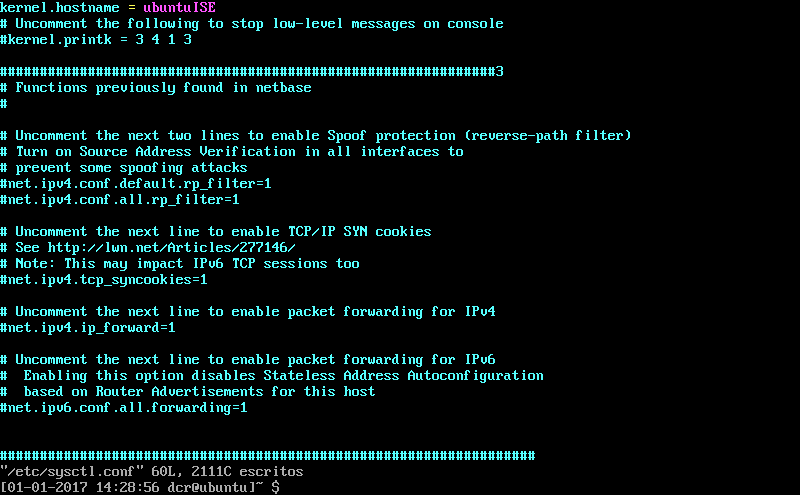
\includegraphics[scale=0.4]{modifySysctl.png}
	\caption{Añadimos el parámetro kernel.hostname y lo nombramos \textit{ubuntuISE}.}
\end{figure}
Tras guardar y modificar el archivo reiniciamos el sistema. Tras volver a arrancar la máquina virtual observamos los cambios tanto en la pantalla de inicio de sesión como a la derecha de la arroba en la terminal como podemos comprobar en la siguiente captura.
\begin{figure}[H]
	\centering
	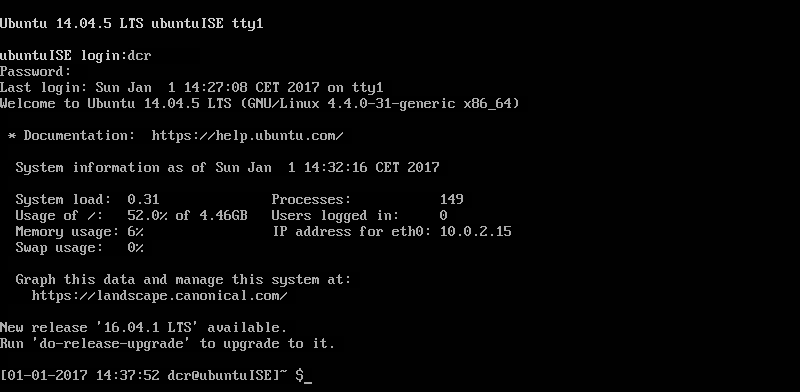
\includegraphics[scale=0.4]{testSysctl.png}
	\caption{Comprobamos que tanto en el inicio de sesión como en la terminal aparece ubuntuISE en vez de ubuntu tras reiniciar el sistema.}
\end{figure}
%----------------------------------------------------------------------------------------
%	Cuestión 2
%----------------------------------------------------------------------------------------
\section{¿Con qué opción se muestran todos los parámetros modificables en tiempo de ejecución? Elija dos parámetros y explique, en dos líneas, qué función tienen.}
Para mostrar todos los parámetros modificables en tiempo de ejecución utilizamos el comando \verb|sysctl -a| \cite{c2}.
\begin{figure}[H]
	\centering
	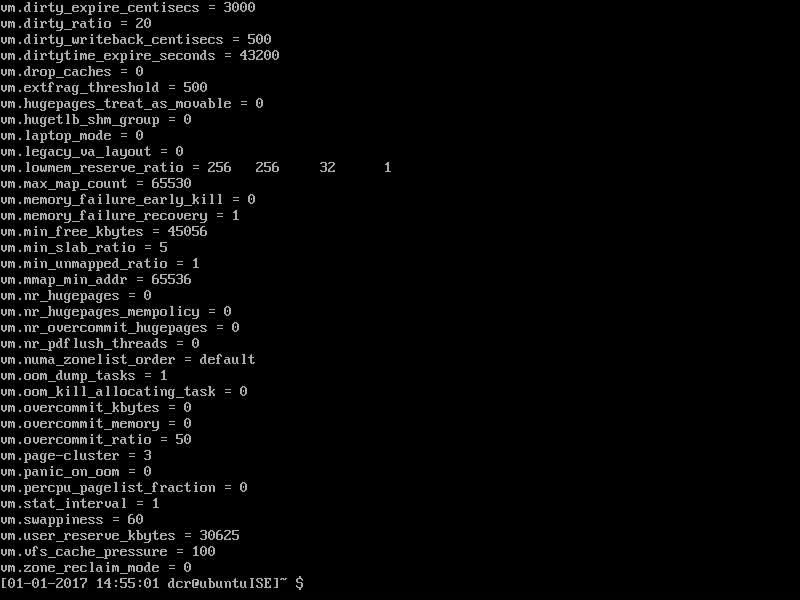
\includegraphics[scale=0.4]{listSysctl.png}
	\caption{Final de la lista de los parámetros modificables en tiempo de ejecución por el comando sysctl en Ubuntu Server 14.04.}
\end{figure}

De la lista voy a escoger los siguientes parámetros:
\begin{itemize}
	\item \textbf{fs.file-max} determina el número máximo de manejadores de archivo abiertos a la vez, por tanto, nos permite alterar el número máximo de archivos abiertos. \cite{c2a}
	\item \textbf{kernel.threads-max} determina el número máximo de hebras que pueden ejecutarse a la vez en el sistema. \cite{c2b}
\end{itemize}
%----------------------------------------------------------------------------------------
%	Cuestión 3
%----------------------------------------------------------------------------------------
\section{Cuestión 3.}
\subsection{Realice una copia de seguridad del registro y restáurela, ilustre el proceso con capturas.}
Siguiendo la información obtenida en \cite{c3}
Realizamos la copia de seguridad exportando los datos del registro.
\begin{figure}[H]
	\centering
	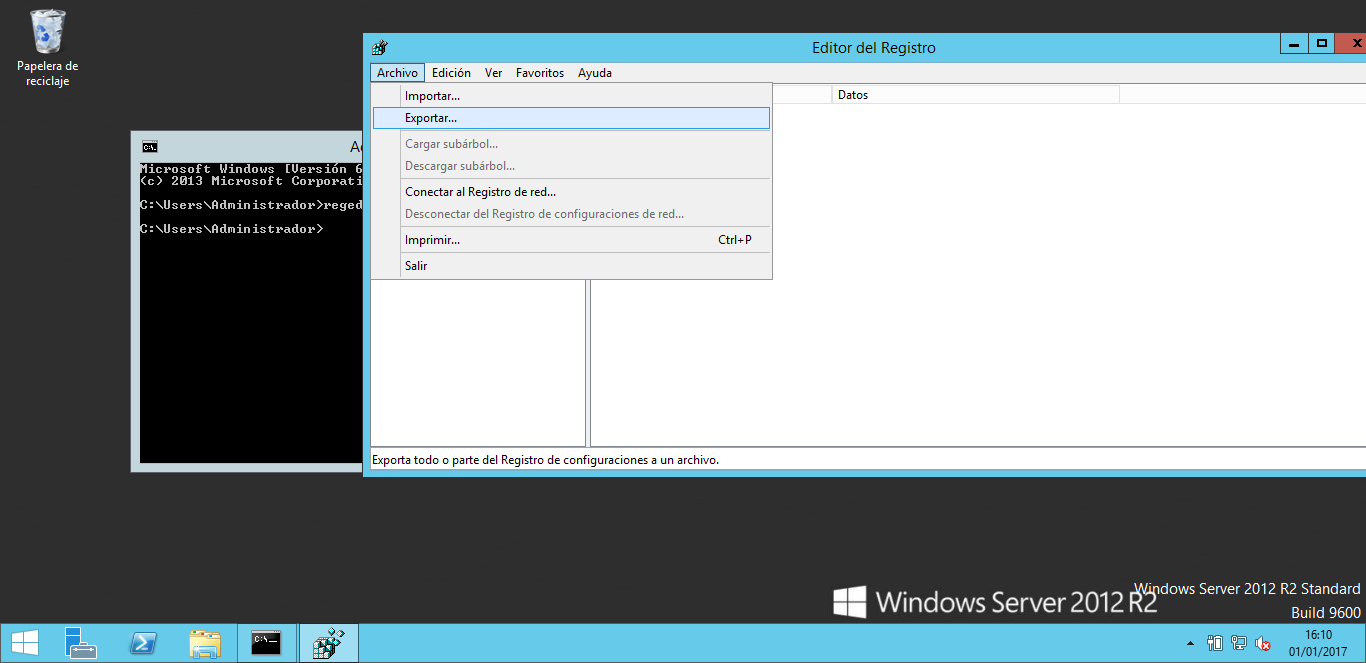
\includegraphics[scale=0.4]{regedit1.png}
	\caption{Una vez abierto el editor del registro marcamos en Archivo > Exportar ...}
\end{figure}

\begin{figure}[H]
	\centering
	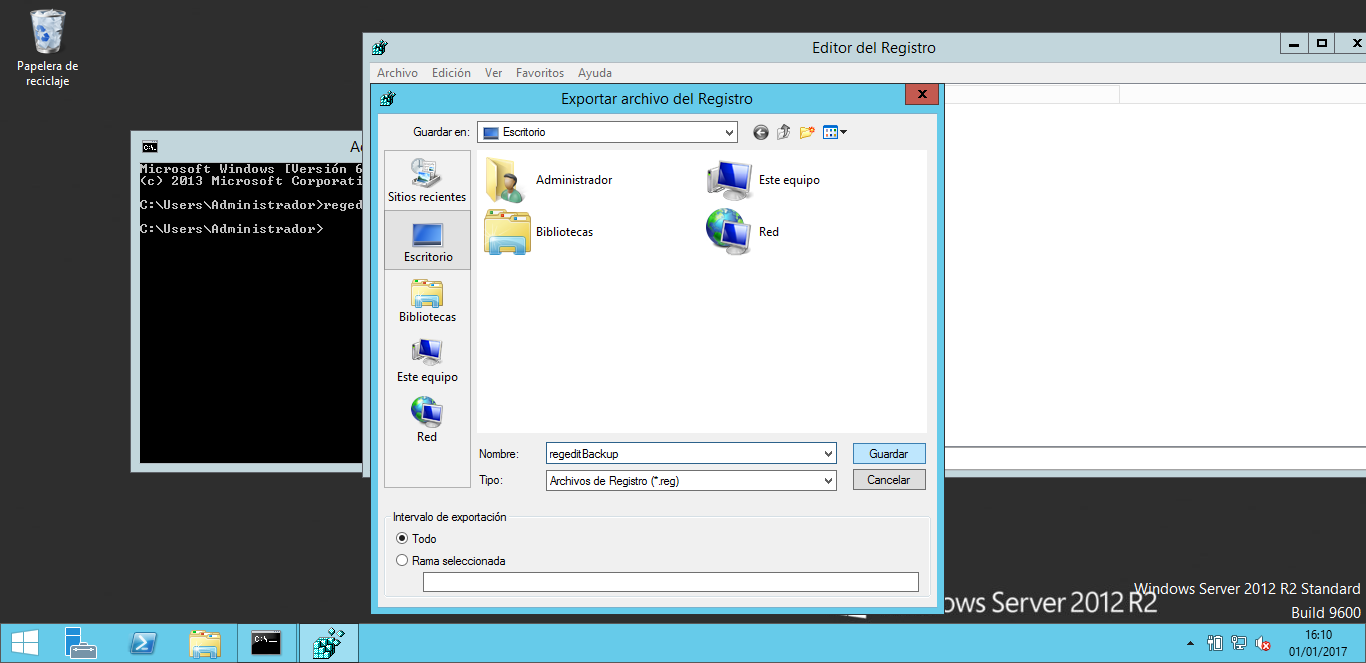
\includegraphics[scale=0.4]{regedit2.png}
	\caption{Seleccionamos el Escritorio como ubicación (para que esté accesible), seleccionando Todo como el intervalo de exportación y nombrándolo regeditBackup y pulsando en Guardar.}
\end{figure}

Para comprobar que realmente funciona, primero modifico un parámetro cualquiera.
\begin{figure}[H]
	\centering
	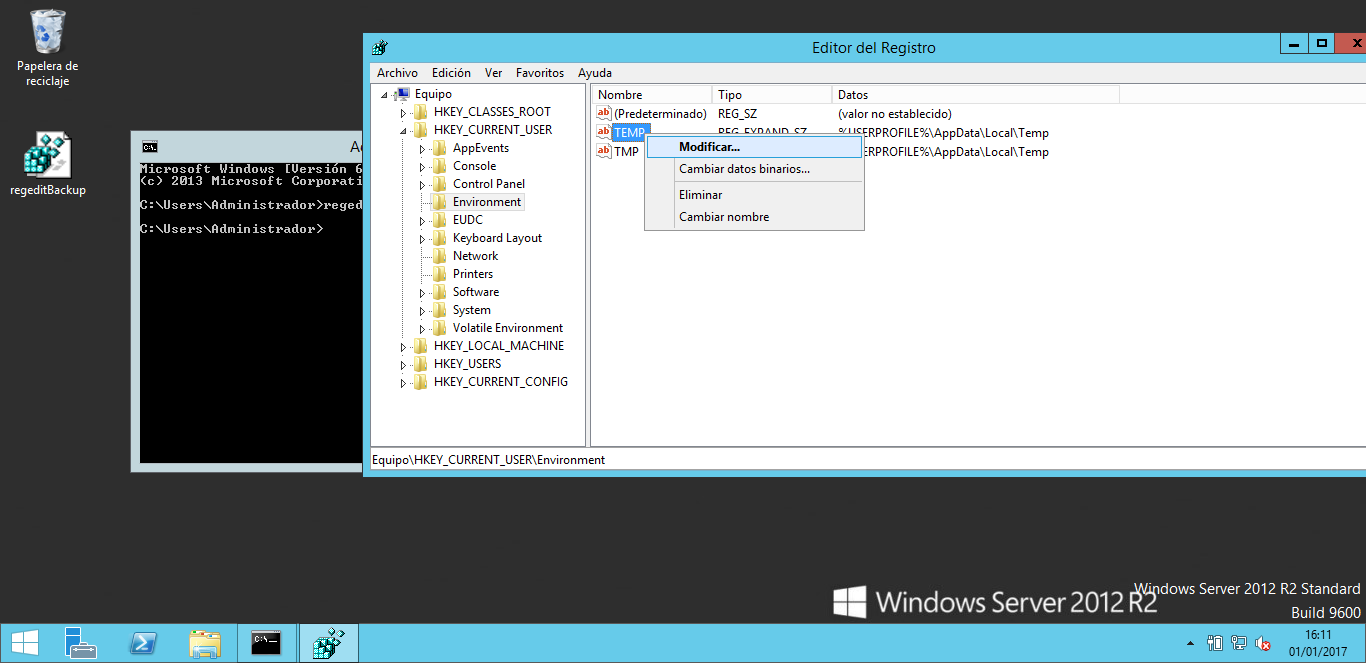
\includegraphics[scale=0.4]{regedit3.png}
	\caption{Haciendo click derecho en el registro HKEY\_CURRENT\_USER/Environment/TEMP pulsamos en Modificar...}
\end{figure}

\begin{figure}[H]
	\centering
	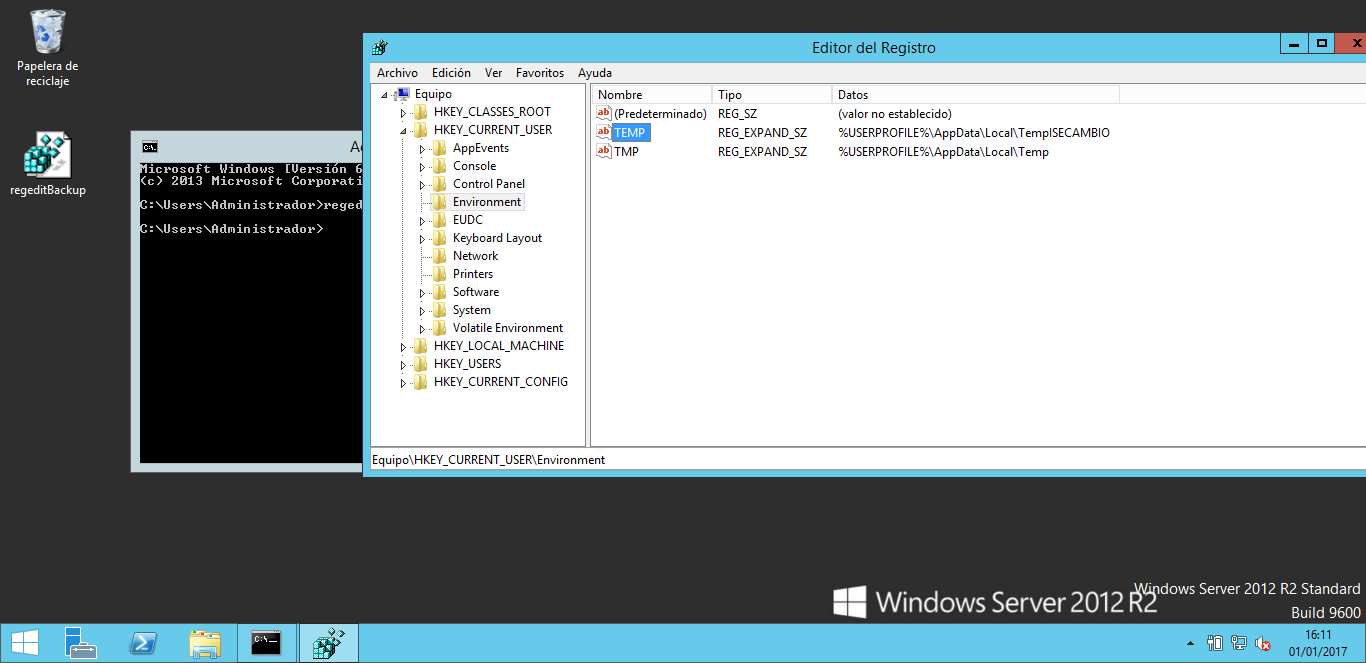
\includegraphics[scale=0.4]{regedit4.png}
	\caption{Tras modificarlo observamos que efectivamente el cambio ha tenido lugar.}
\end{figure}

Para restaurar el estado importamos del archivo previamente guardado.

\begin{figure}[H]
	\centering
	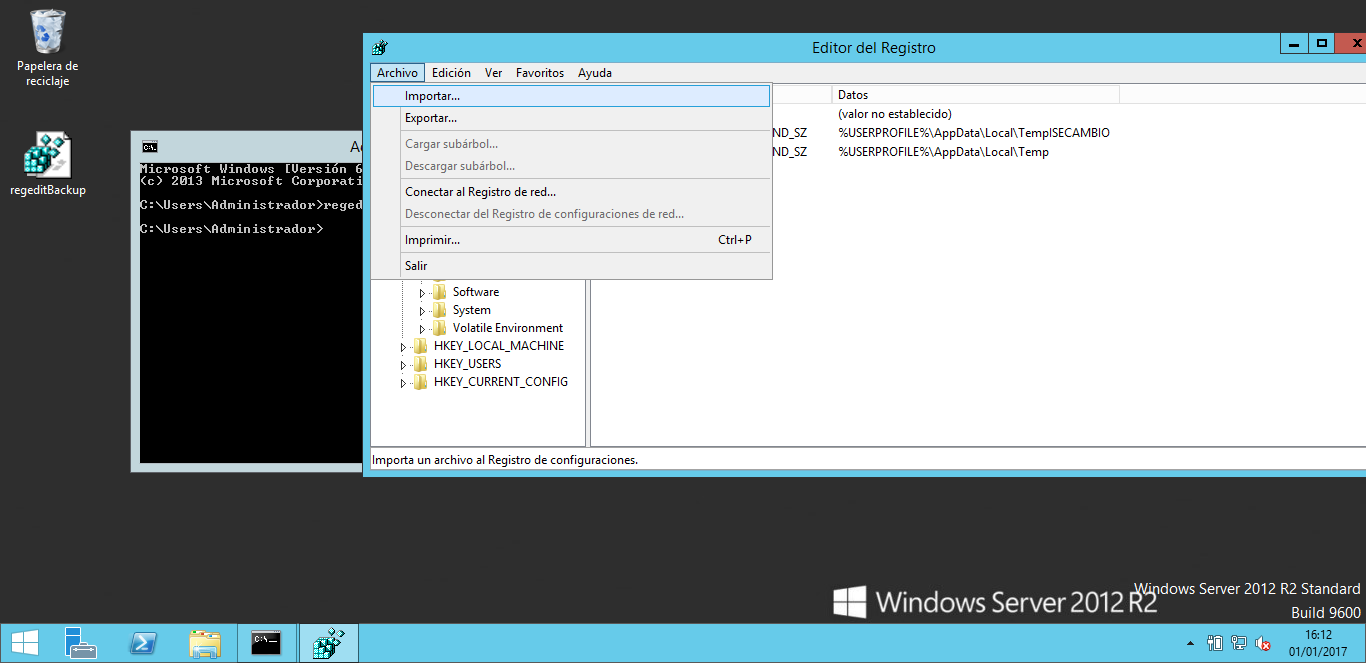
\includegraphics[scale=0.4]{regedit5.png}
	\caption{En el editor del registro marcamos Archivo > Importar ...}
\end{figure}


\begin{figure}[H]
	\centering
	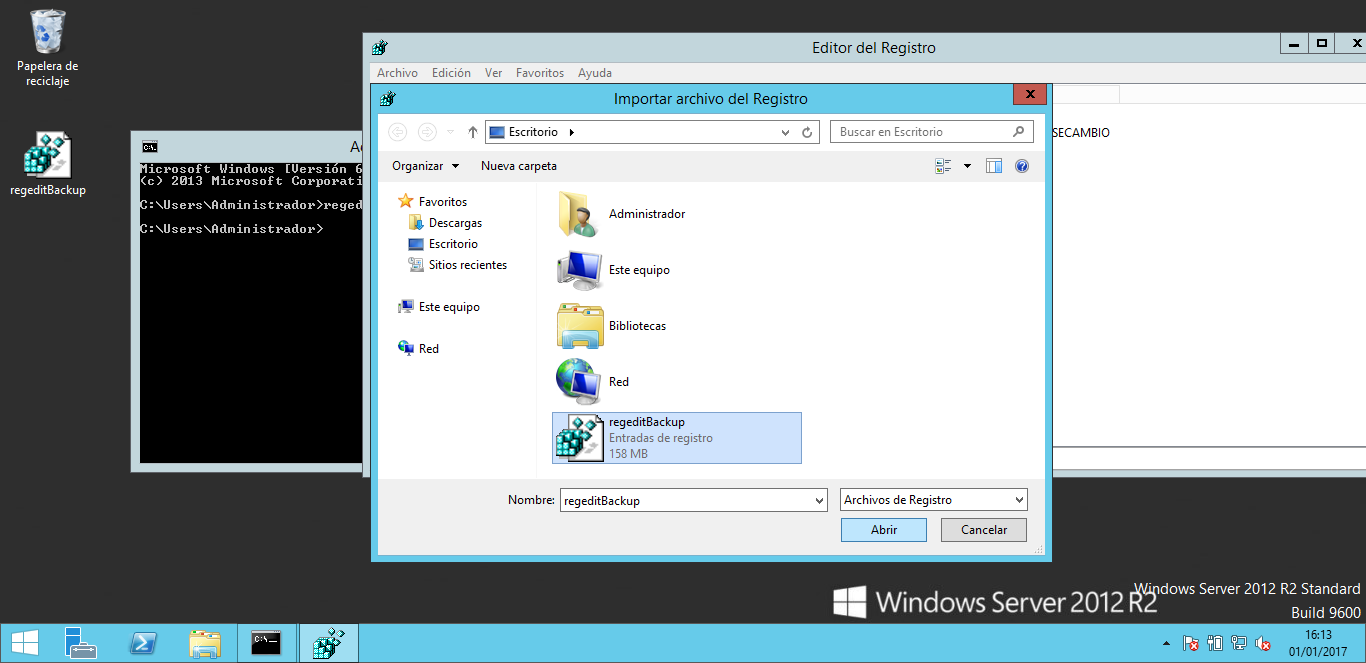
\includegraphics[scale=0.4]{regedit6.png}
	\caption{Seleccionamos la copia de seguridad hecha previamente ubicada en el escritorio.}
\end{figure}

\begin{figure}[H]
	\centering
	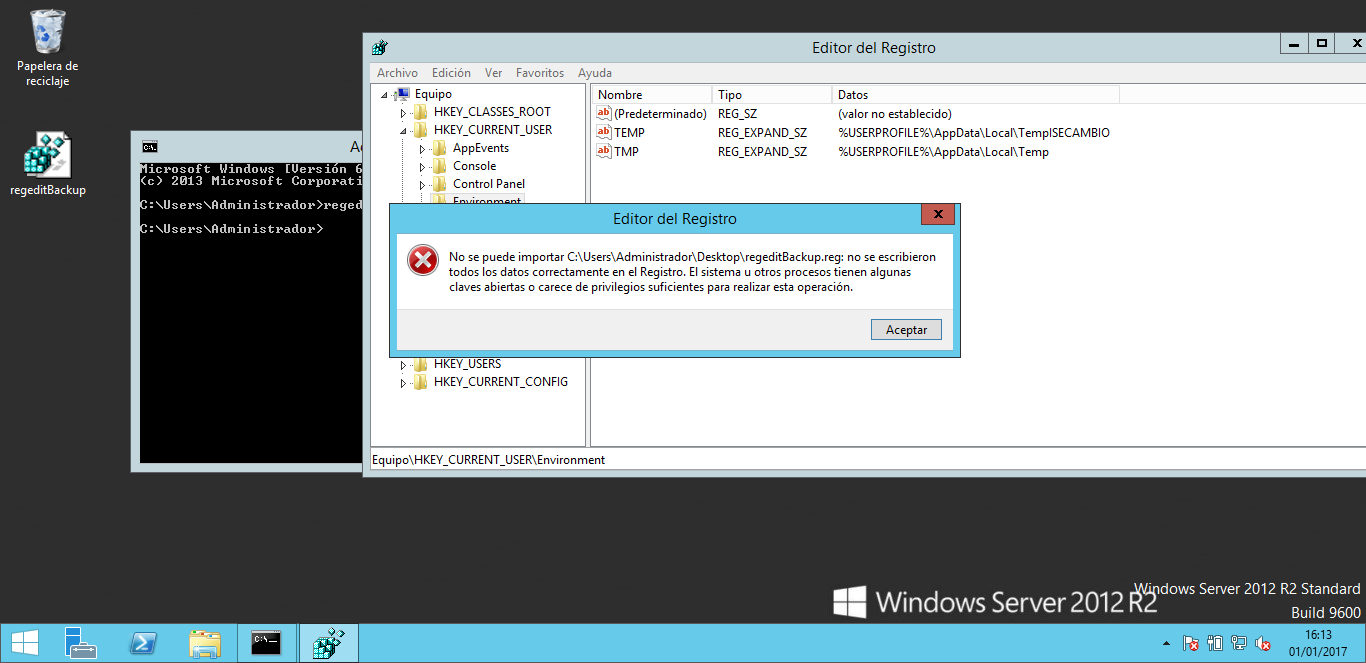
\includegraphics[scale=0.4]{regedit7.png}
	\caption{Obtenemos un error puesto que no podemos modificar los registros que estén siendo usados por algunos programas o no tenemos permisos.}
\end{figure}

\begin{figure}[H]
	\centering
	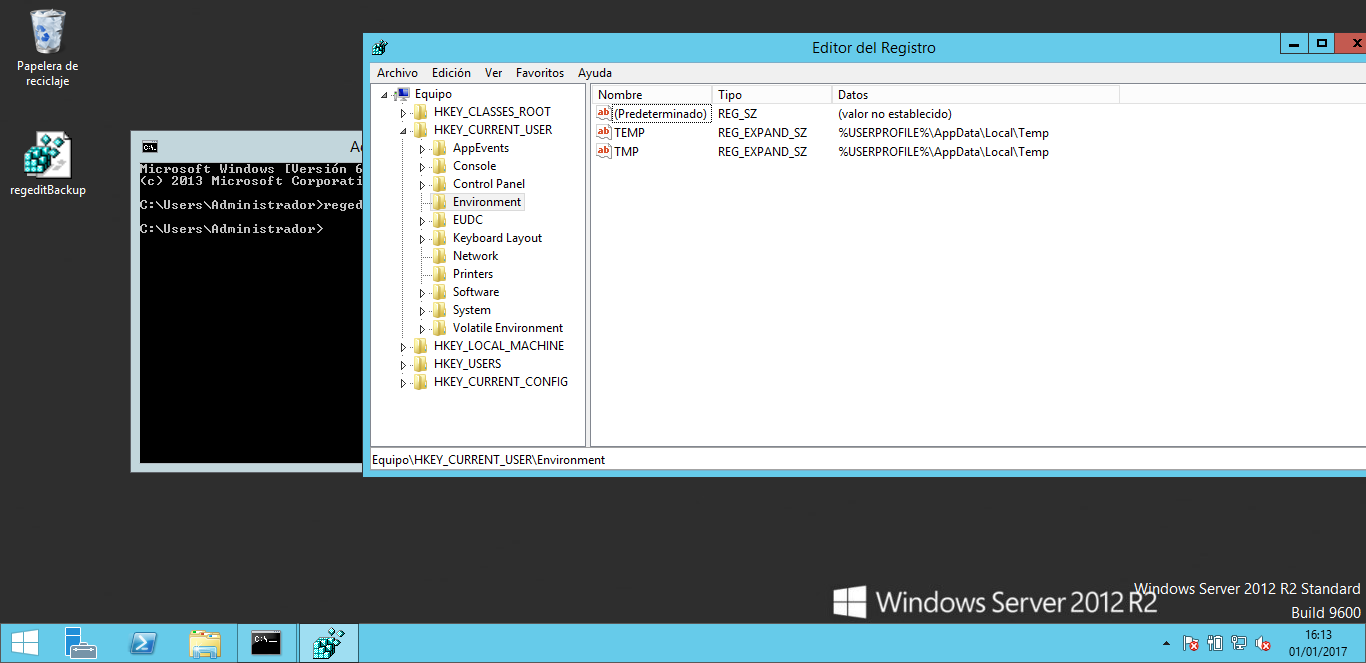
\includegraphics[scale=0.4]{regedit8.png}
	\caption{Observamos que el valor modificado ha vuelto a su valor inicial.}
\end{figure}
\subsection{Abra una ventana mostrando el editor del registro.}
Basándonos en la información proporcionada por el guión es fácil abrir una ventana del editor del registro, para ello seguimos los siguiente pasos:

\begin{figure}[H]
	\centering
	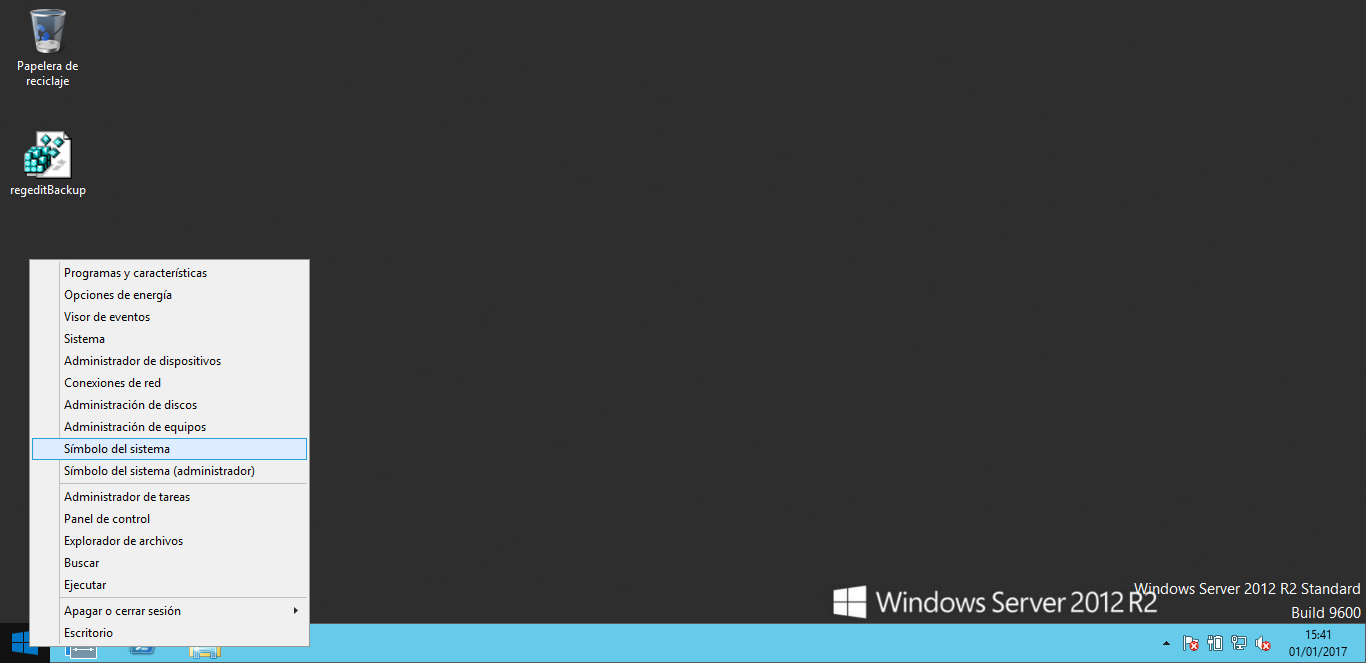
\includegraphics[scale=0.4]{openregedit1.png}
	\caption{Haciendo click derecho en el dibujo de inicio seleccionamos \textit{Símbolo del sistema}.}
\end{figure}

\begin{figure}[H]
	\centering
	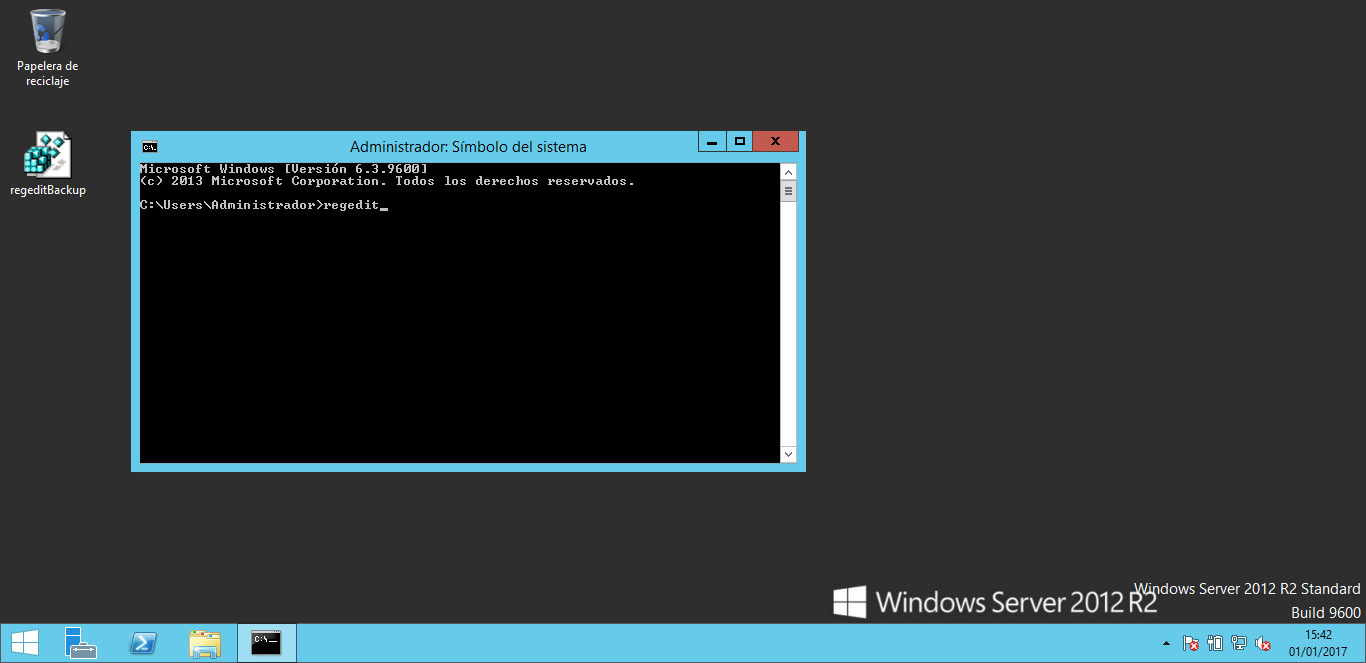
\includegraphics[scale=0.4]{openregedit2.png}
	\caption{En el símbolo del sistema utilizamos el comando \textit{regedit}.}
\end{figure}

\begin{figure}[H]
	\centering
	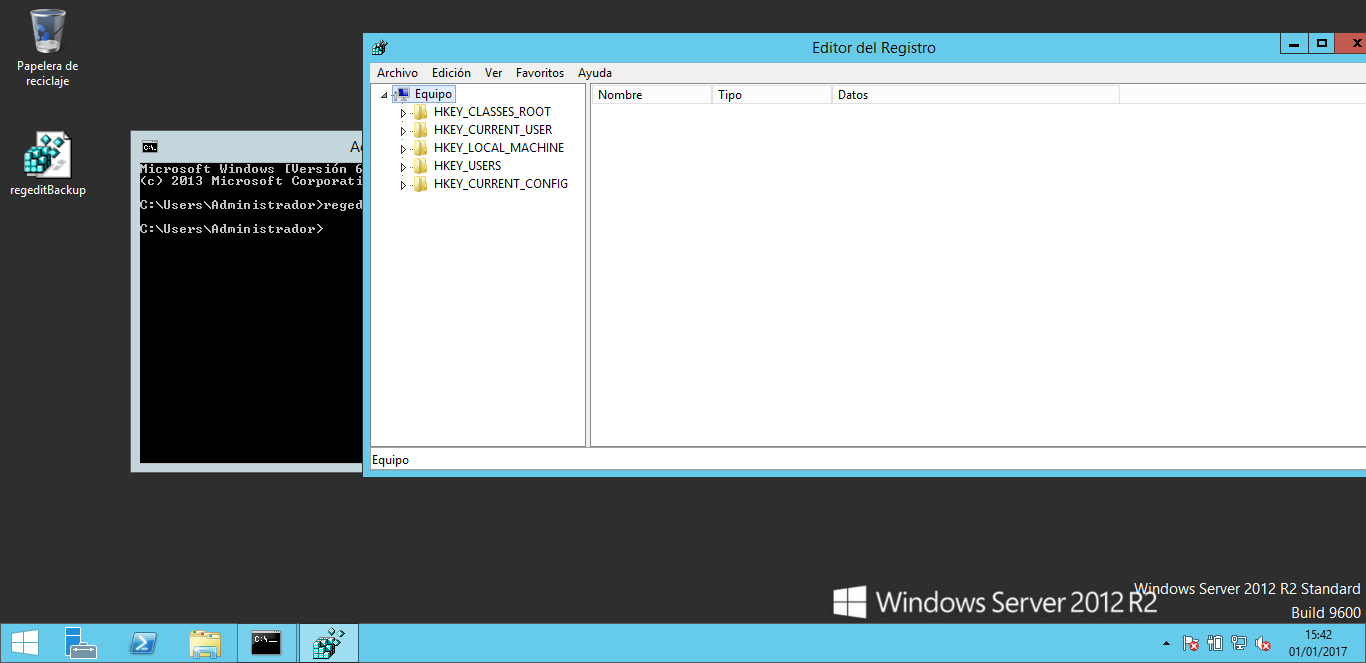
\includegraphics[scale=0.4]{openregedit3.png}
	\caption{Se abre una ventana del editor del registro.}
\end{figure}

%----------------------------------------------------------------------------------------
%	Cuestión 4
%----------------------------------------------------------------------------------------
\section{Enumere qué elementos se pueden configurar en Apache y en IIS para que Moodle funcione mejor.}
Según la información encontrada en \cite{c4} podemos configurar los siguientes elementos:
\subsection{Apache}
\begin{itemize}
	\item Número máximo de procesos hijos que se crearán para atender a un cliente (MaxClients).
	\item Número máximo de peticiones que puede atender un proceso hijo (MaxRequestsPerChild).
	\item Bajar el tiempo de espera o desactivar las conexiones HTTP \textit{(Hypertext Transfer Protocol)} persistentes (KeepAlive Off | KeepAliveTimeout)
	\item Si no se usa .htaccess, \textit{AllowOverride}.
	\item Evitar la negociación de contenido con \textit{DirectoryIndex}.
	\item Deshabilitar toda la información y estado extra ExtendedStatus Off, \textit{mod\_info} y \textit{mod\_status}.
	\item Bajar la latencia del DNS deshabilitando \textit{HostnameLookups}.
	\item Reducir el uso de I/O con \textit{Options -Index FollowSymLinks} y evitando Multiviews.
	\item Tiempo que ha de transcurrir para que falle una petición (TimeOut).
\end{itemize}
\subsection{IIS}
\begin{itemize}
	\item Tiempo de espera de conexiones persistentes (ListenBackLog).
	\item Ajustar el tamaño máximo de archivos en caché (MemCacheSize).
	\item Ajustar el tamaño máximo de un archivo en caché (MemCachedFileSize).
	\item Tiempo que algo es guardado en caché (ObjectCacheTTL).
\end{itemize}
%----------------------------------------------------------------------------------------
%	Cuestión 5
%----------------------------------------------------------------------------------------
\section{Ajuste la compresión en el servidor y analice su comportamiento usando varios valores para el tamaño del archivo a partir del cuál comprimir. Para comprobar que está comprimiendo puede usar el navegador o comandos como curl (see url) o lynx. Muestre capturas de todo el proceso.}

\begin{figure}[H]
	\centering
	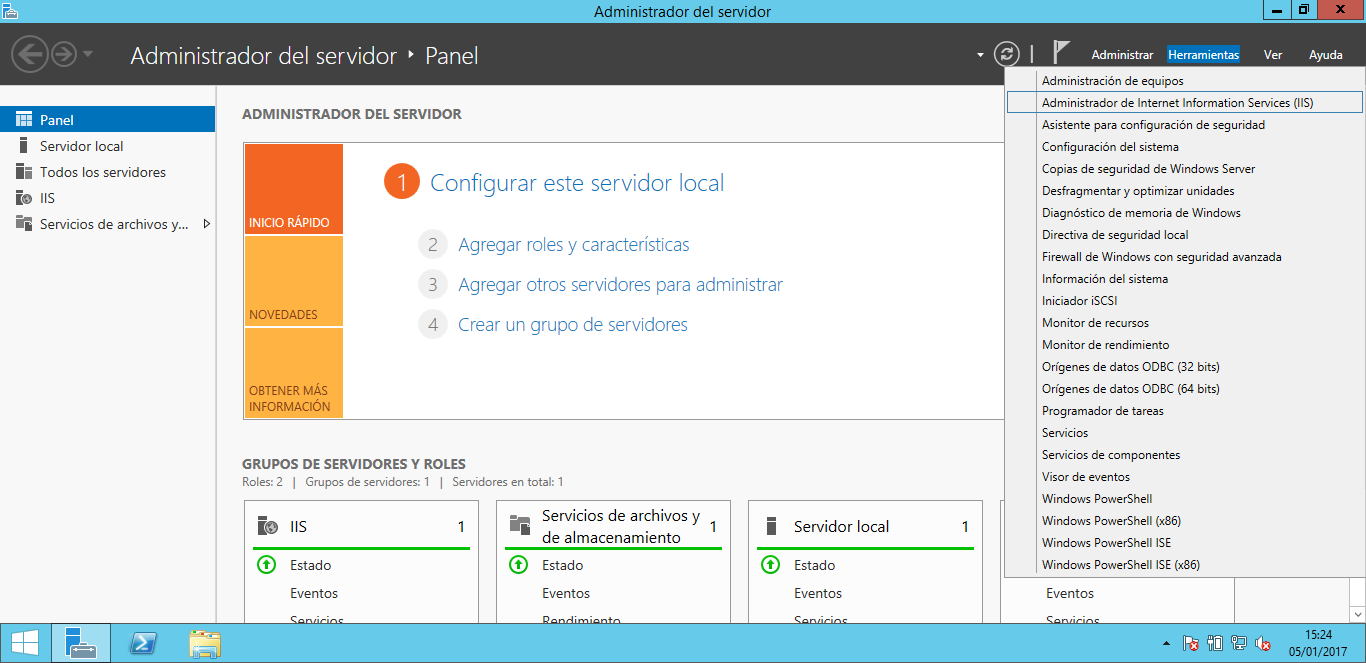
\includegraphics[scale=0.4]{iis1.png}
	\caption{En el administrador del servidor pulsamos en Herramientas > \space Administrador de Internet Informacion Services (IIS).}
\end{figure}

\begin{figure}[H]
	\centering
	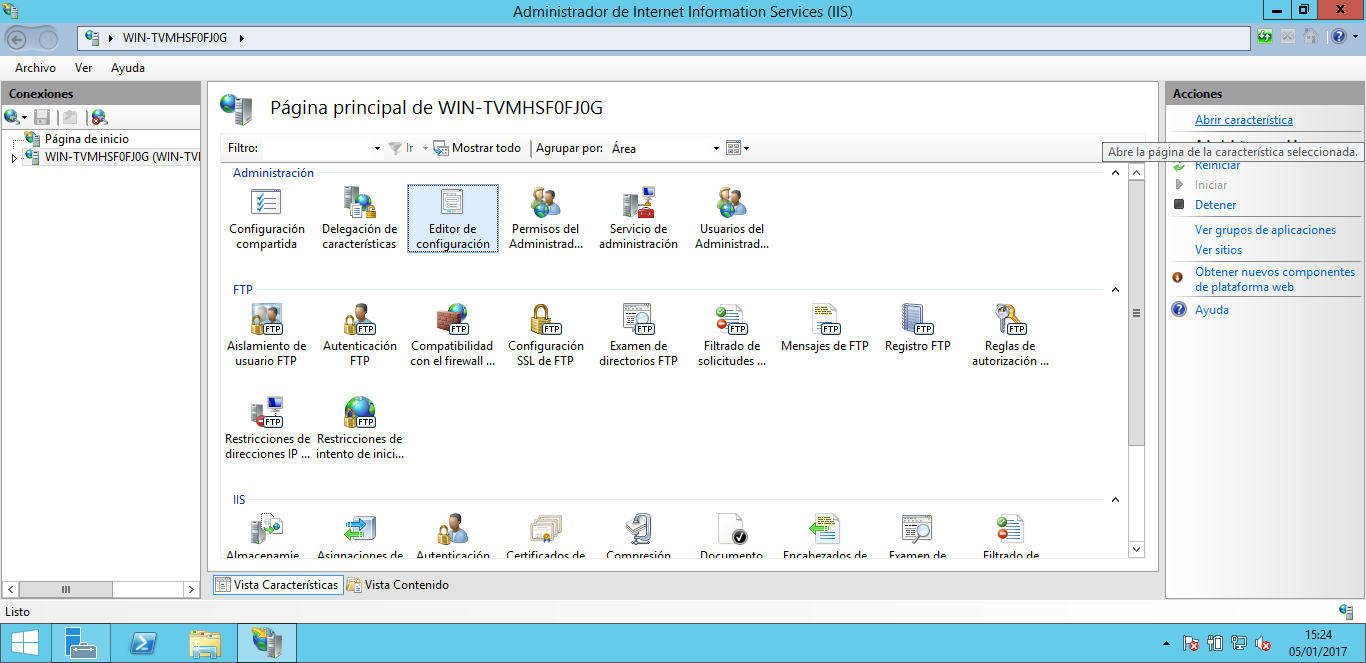
\includegraphics[scale=0.4]{iis2.png}
	\caption{Escogiendo en la izquierda el servidor pulsamos en editor de configuración y pulsamos en abrir característica.}
\end{figure}

\begin{figure}[H]
	\centering
	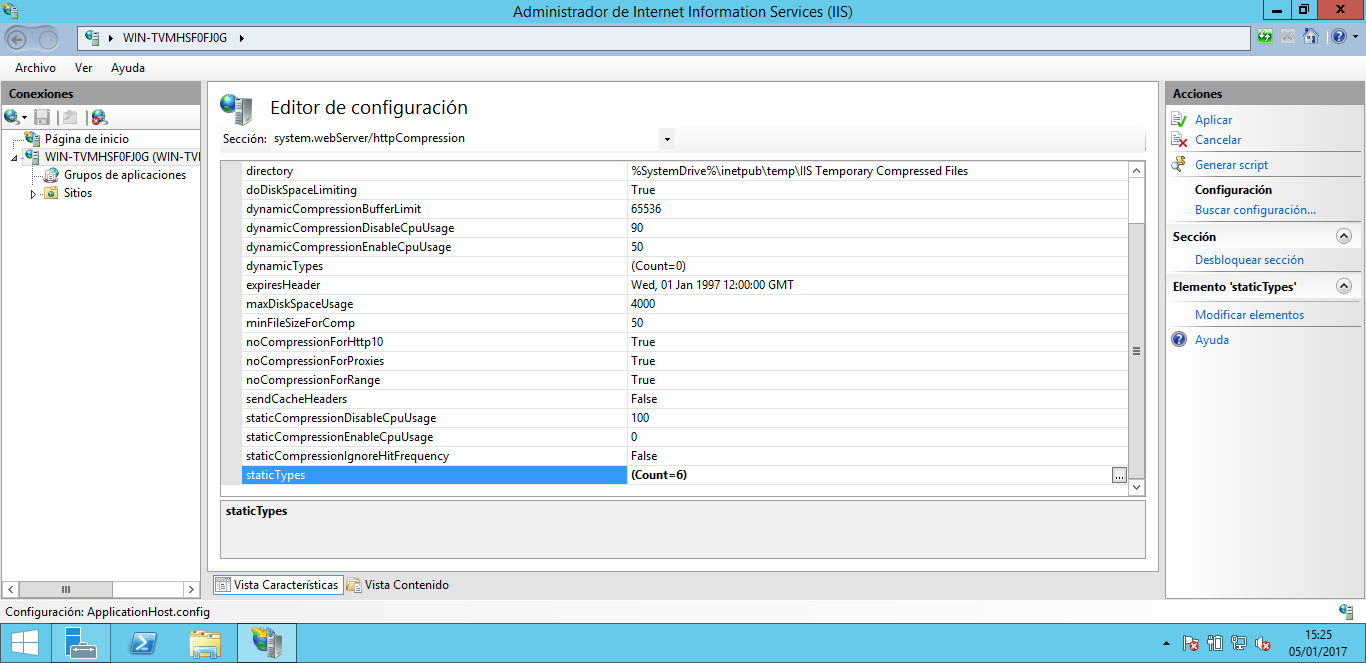
\includegraphics[scale=0.4]{iis3.png}
	\caption{Arriba escogemos en system.webServer/httpCompression y configuramos los valores referentes a la compresión estática.}
\end{figure}
Los parámetros que podemos configurar son los relacionados con la compresión estática \cite{c5} para que funcione siempre y comprima la página por defecto de IIS en Window Server 2012 R2
\begin{itemize}
	\item \textbf{maxDiskSpaceUsage} - Tamaño máximo (en MB) que pueden ocupar en disco los archivos comprimidos
	\item \textbf{minFileSizeForComp} - Tamaño mínimo que ha de tener el archivo para que sea comprimido
	\item \textbf{staticCompressionDisableCpuUsage} - Uso de CPU que implica que se desactive la compresión estática.
	\item \textbf{staticCompressionEnableCpuUsage} - Uso de CPU que implica que se active la compresión estática
	\item \textbf{staticTypes} - Lista de tipos MIME (Multipurpose Internet Mail Extensions) y sus valores booleanos para indicar si se deben comprimir o no.
\end{itemize}


\begin{figure}[H]
	\centering
	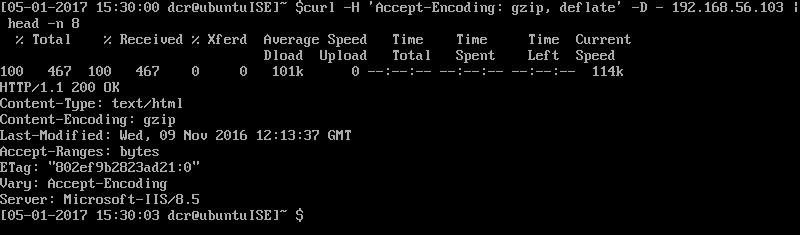
\includegraphics[scale=0.6]{iis4.png}
	\caption{Con curl desde la máquina virtual de Ubuntu Server 14.04 comprobamos que efectivamente llega comprimido (gzip).}
\end{figure}

\begin{figure}[H]
	\centering
	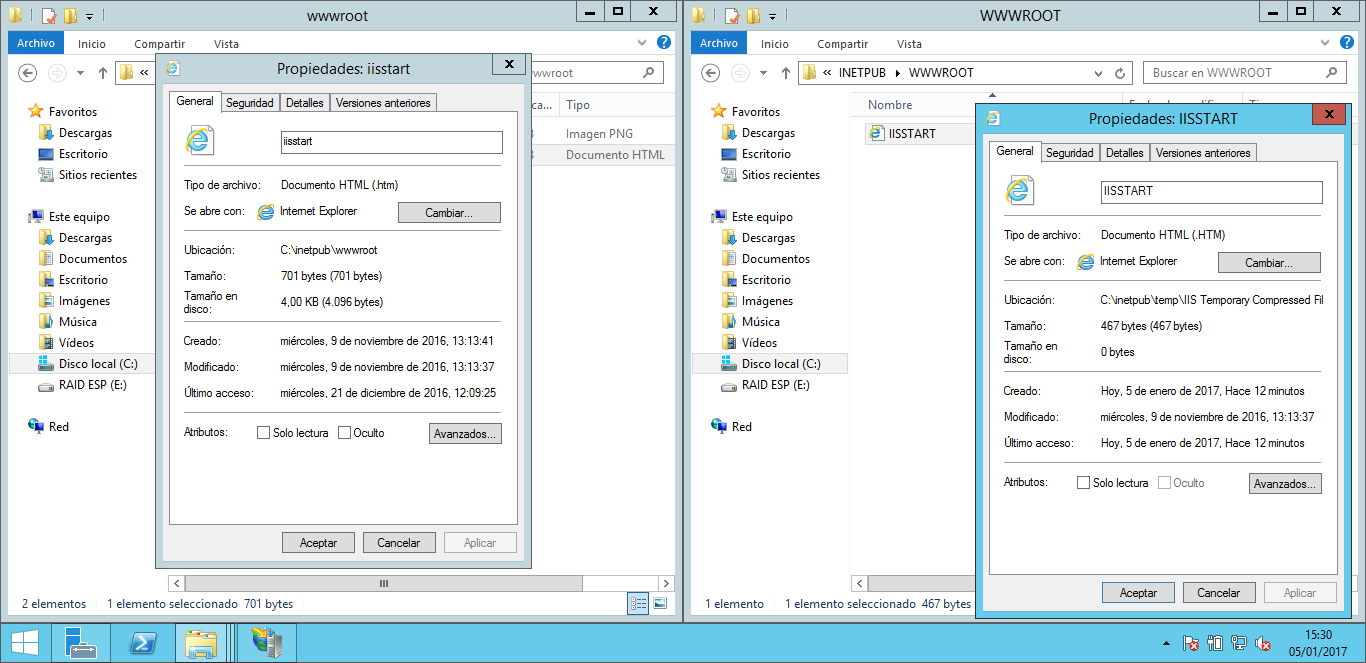
\includegraphics[scale=0.4]{iis5.png}
	\caption{A la izquierda directorio web con información del archivo sin comprimir. A la derecha directorio de compresión con información del archivo principal comprimido.}
\end{figure}

\begin{figure}[H]
	\centering
	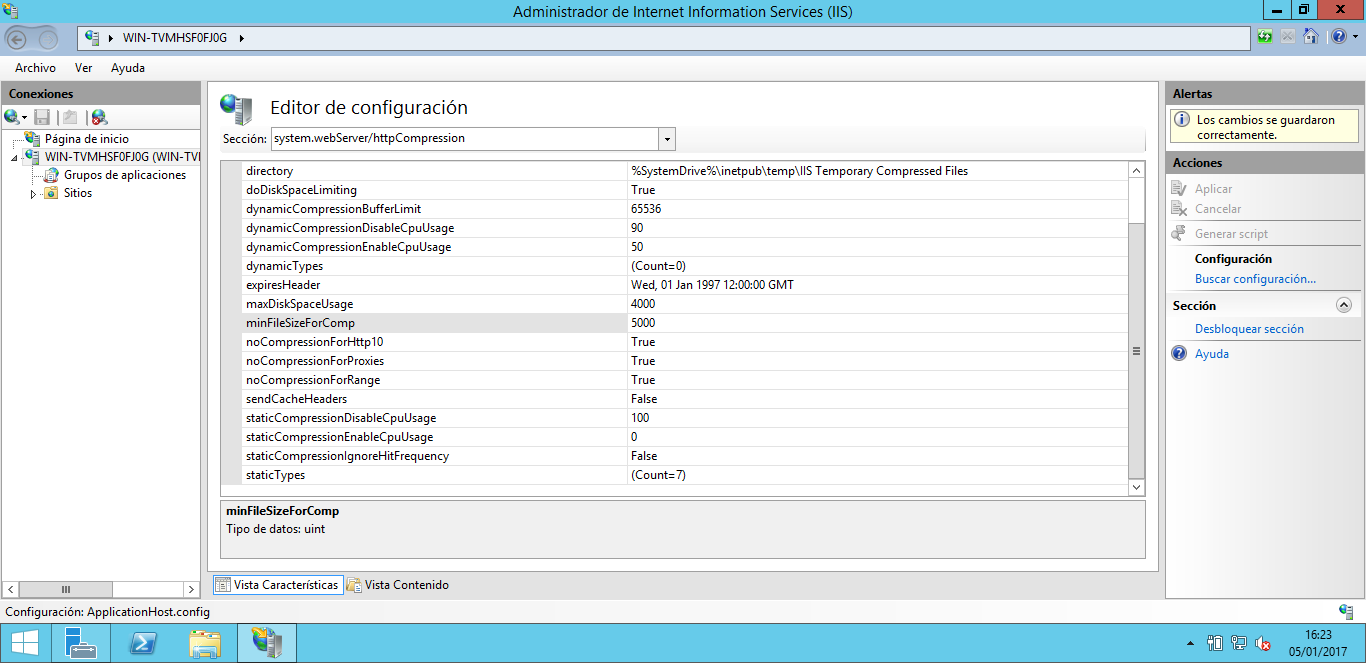
\includegraphics[scale=0.4]{iis6.png}
	\caption{Ahora activamos la compresión solo para archivos mayores a 5000 bytes.}
\end{figure}

\begin{figure}[H]
	\centering
	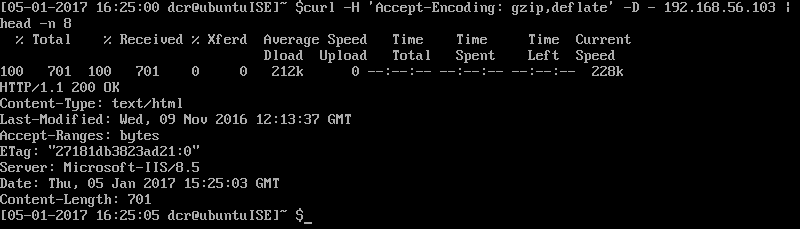
\includegraphics[scale=0.6]{iis7.png}
	\caption{Con curl desde la máquina virtual de Ubuntu Server 14.04 comprobamos que efectivamente ahora no se ha comprimido (ya que sólo pesa 701 bytes).}
\end{figure}
%----------------------------------------------------------------------------------------
%	Cuestión 6
%----------------------------------------------------------------------------------------
\section{Cuestión 6.}
\subsection{Usted parte de un SO con ciertos parámetros definidos en la instalación (Práctica 1), ya sabe instalar servicios (Práctica 2) y cómo monitorizarlos (Práctica 3) cuando los somete a cargas (Práctica 4). Al igual que ha visto cómo se puede mejorar un servidor web (Práctica 5 Sección 3.1), elija el servicio (el que usted quiera) y modifique un parámetro para mejorar su comportamiento.}
En mi caso he decidido que voy a realizar el cambio sobre el servidor web Apache que tengo en mi máquina virtual con CentOS y modificando el parámetro Max-Clients explicado anteriormente. Para realizar la monitorización utilizaré Apache Benchmark desde mi máquina virtual con Ubuntu Server.
\subsection{Monitorice el servicio antes y después de la modificación del parámetro aplicando cargas al sistema (antes y después) mostrando los resultados de la monitorización.}
Para empezar realizamos la monitorización del sistema antes de realizar la modificación del parámetro. Para ello utilizamos Apache Benchmark con una concurrencia de 5 y un número de peticiones de 120000.

\begin{figure}[H]
	\centering
	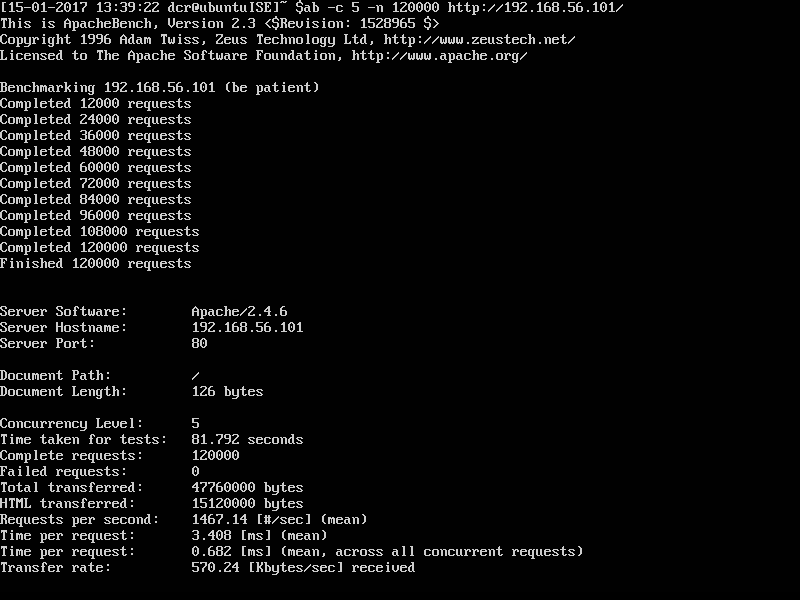
\includegraphics[scale=0.6]{abPrevio1.png}
	\caption{Ejecución de \textit{ab} desde Ubuntu Server 14.04 contra el servidor web de CentOS antes de la modificación.}
\end{figure}

Para realizar la modificación del parámetro hemos de modificar el archivo httpd.conf ubicando en /etc/httpd/conf. El parámetro que voy a modificar es MaxClients, que determina el número máximo de peticiones simultáneas que Apache va a tratar \cite{c6}. Puesto que no he sido capaz de averiguar cuál es el valor por defecto de la directiva MaxClients para mi versión de Apache en CentOS, supongo que será aproximadamente las 75 hebras que en la práctica anterior vi que creaba Apache al aplicarle la carga así que determino que voy a darle un valor de 100 para poder mejorar el tráfico atendido ya que la máquina virtual tiene recursos más que de sobra para poder atender más peticiones.

\begin{figure}[H]
\centering
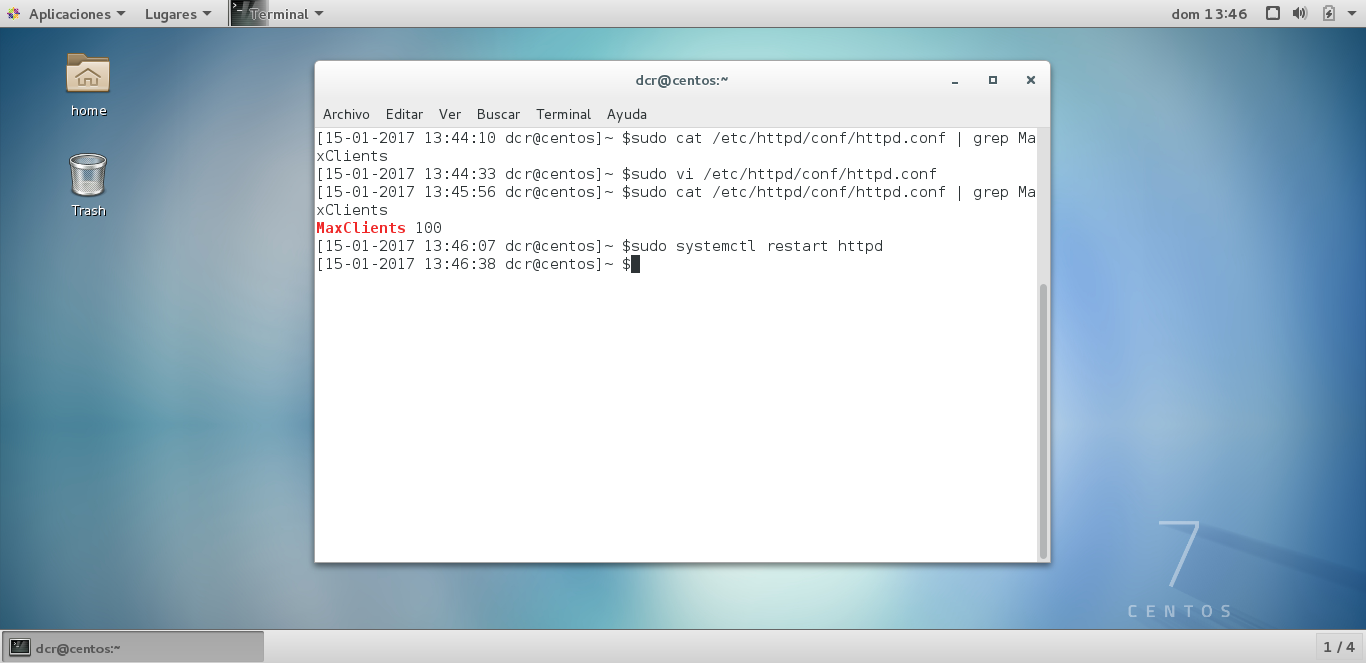
\includegraphics[scale=0.6]{modifyParameter.png}
\caption{Ponemos el valor de la directiva MaxClients en el archivo de configuración de httpd.}
\end{figure}

Tras hacer la modificación volvemos a monitorizar con Apache Benchmark y obtenemos los siguientes resultados:

\begin{figure}[H]
	\centering
	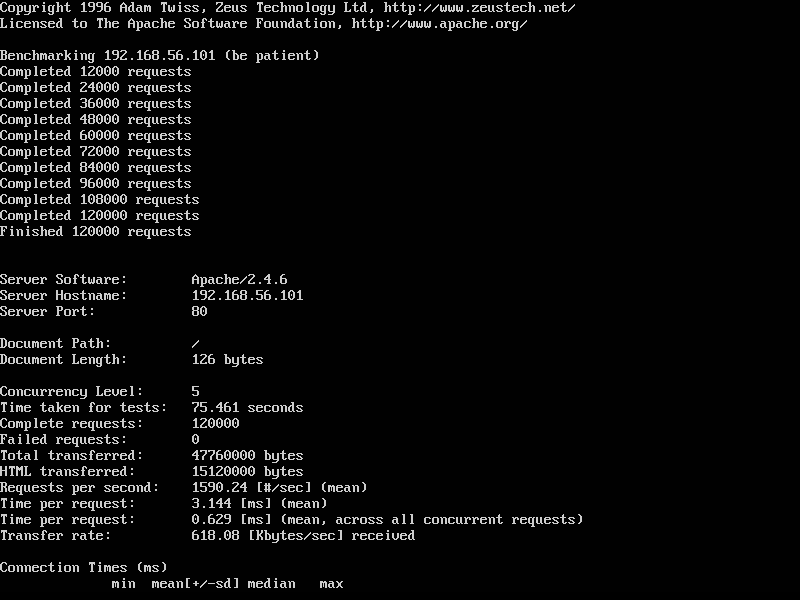
\includegraphics[scale=0.6]{abPosterior1.png}
	\caption{Ejecución de \textit{ab} desde Ubuntu Server 14.04 contra el servidor web de CentOS después de la modificación.}
\end{figure}

Como podemos observar la productividad media ha aumentado mirado el campo ```requests per second'' en algo más de 100 peticiones por segundo. Por tanto considero que el cambio ha sido beneficioso para el servidor web y a falta de experimentar con más detalle para obtener un valor óptimo, es mejor poner la directiva MaxClients a 100 que dejarla en su valor por defecto.
%----------------------------------------------------------------------------------------
%	Bibliografía
%----------------------------------------------------------------------------------------
\bibliography{citas} %archivo citas.bib que contiene las entradas 
\bibliographystyle{ieeetr} % hay varias formas de citar
\end{document}
